\chapter{Praktische Anwendung von SHAP auf lineare Modelle}

In diesem Kapitel wird der Einsatz des SHAP-Frameworks zur Interpretation linearer Modelle im 
Kontext des maschinellen Lernens untersucht. Lineare Modelle, gekennzeichnet durch ihre Transparenz 
und einfache Struktur, bilden oft die Basis für das Verständnis komplexerer Algorithmen. 
Dennoch bleibt die Herausforderung bestehen, die Beiträge individueller Merkmale zur Modellvorhersage zu 
quantifizieren und zu interpretieren.

Die Anwendung von SHAP-Werten ermöglicht es, diesen Herausforderungen zu begegnen und Einblicke in 
die Modellvorhersagen zu gewähren, die über traditionelle Methoden hinausgehen. 
Dieses Kapitel führt in die Grundlagen des \textsf{shap}-Pakets ein, demonstriert dessen Anwendung auf einen 
spezifischen Datensatz und diskutiert die Berechnung sowie Interpretation der resultierenden SHAP-Werte. 
Die daraus gewonnenen Erkenntnisse leisten einen Beitrag zur Erklärbarkeit von Vorhersagemodellen und 
unterstützen somit die wissenschaftliche Diskussion um die Verantwortlichkeit und Nachvollziehbarkeit 
in der maschinellen Lernforschung.

\section{Lineare Modelle als analytische Grundlage}

In linearen Regressionsmodellen wird die Zielgröße als eine gewichtete Kombination der Eingangsmerkmale bestimmt. 
Die einfache lineare Struktur dieser Modelle erleichtert das Verständnis der Beziehungen zwischen den Eingangsdaten 
und den Vorhersagen. 

Lineare Modelle sind ein grundlegendes Werkzeug in der statistischen Modellierung und dienen dazu, das Verhältnis zwischen 
einer abhängigen Variablen, die üblicherweise mit $y^{(i)}$ bezeichnet wird, 
und einem oder mehreren Prädiktoren, den unabhängigen Variablen $x_i$, zu erfassen. 
Diese Beziehungen werden mittels linearer Gleichungen dargestellt, die für jede 
einzelne Beobachtung $i$ im Datensatz folgendermaßen formuliert werden können:

\begin{equation}
    y^{(i)} = \beta_0 + \sum_{j=1}^{p} \beta_j x^{(i)}_j + \epsilon^{(i)},
\end{equation}

wobei das Ergebnis, das von einem linearen Modell für eine gegebene Beobachtung vorhergesagt wird, sich als Summe der mit 
Gewichten $\beta_j$ versehenen Merkmale $p$ ergibt.

Hierbei stellt $y^{(i)}$ den beobachteten Wert der abhängigen Variablen für die Beobachtungseinheit
$i$ dar. Der Term $\beta_0$ ist der Achsenabschnitt oder y-Achsenabschnitt des Modells, 
welcher den erwarteten Wert von $y$ darstellt, wenn alle unabhängigen Variablen $x$ null sind. 
Die Summe $\sum_{j=1}^{p} \beta_j x^{(i)}_j$ berechnet sich aus den Produkten der Koeffizienten 
$\beta_j$ und den Werten der unabhängigen Variablen $x^{(i)}_j$ für jede Beobachtungseinheit $i$ 
und jeden Prädiktor $j$, wobei die Koeffizienten $\beta_j$ den geschätzten Einfluss der 
entsprechenden unabhängigen Variablen auf die abhängige Variable beschreiben.

Der Fehlerterm $\epsilon^{(i)}$ steht für die Residuen, also die Differenzen zwischen den beobachteten 
und durch das Modell geschätzten Werten von $y^{(i)}$. Es wird angenommen, dass diese Fehler normalverteilt sind, 
was bedeutet, dass Abweichungen in beiden Richtungen um den Mittelwert (hier Null) 
mit abnehmender Wahrscheinlichkeit für größere Fehler auftreten \cite[S. 37]{Molnar_2022}.

In einem linearen Modell stellt der Achsenabschnitt die Basislinie dar, an der die Auswirkungen aller 
anderen Merkmale gemessen werden. Dieser Wert gibt an, was das Modell für die Zielvariable vorhersagen 
würde, wenn alle anderen Merkmale nicht vorhanden wären – der Ausgangspunkt der Vorhersage 
für einen Datensatz, in dem alle anderen Variablen auf null gesetzt sind. 
Es ist wichtig zu erwähnen, dass der Achsenabschnitt für sich genommen nicht immer eine praktische 
Bedeutung hat, da es selten vorkommt, dass alle Variablen tatsächlich den Wert null annehmen. 
Die wahre Aussagekraft des Achsenabschnitts tritt zutage, wenn die Daten so standardisiert wurden, 
dass ihre Mittelwerte bei null und die Standardabweichung bei eins liegen. Unter diesen Umständen repräsentiert der Achsenabschnitt 
die erwartete Zielvariable für einen hypothetischen Fall, in dem alle Merkmale ihren Durchschnittswert 
aufweisen.

Bei der Betrachtung einzelner Merkmale innerhalb des Modells sagt das Gewicht $\beta_j$ eines Merkmals, 
um wie viel sich die Zielvariable $y^{(i)}$ ändert, wenn das Merkmal $x^{(i)}_j$ um eine Einheit erhöht wird – und zwar unter 
der Annahme, dass alle anderen Merkmale unverändert bleiben. 
Dies ermöglicht es, den isolierten Effekt eines jeden Merkmals auf die Vorhersage zu verstehen \cite[S. 39]{Molnar_2022}.

Die optimalen Gewichte, oder Koeffizienten, eines linearen Regressionsmodells werden üblicherweise durch ein Verfahren bestimmt, 
das als Methode der kleinsten Quadrate (engl. \textit{Ordinary Least Squares}, OLS) bekannt ist. 
Diese Methode sucht die Koeffizienten \( \beta_0, \ldots, \beta_p \), welche die Summe der quadrierten 
Differenzen zwischen den beobachteten Werten der Zielvariablen \( y^{(i)} \) und den von dem Modell 
vorhergesagten Werten minimieren:

\begin{equation}
    \hat{\beta} = \arg \underset{\beta_0, \ldots, \beta_p}{\min} \ \sum_{i=1}^{n} \left( y^{(i)} - \left( \beta_0 + \sum_{j=1}^{p} \beta_j x_j^{(i)}\right)\right)^2.
\end{equation}

Das Ergebnis der Minimierung, \( \hat{\beta} \) stellt den Vektor der geschätzten Koeffizienten dar \cite[S. 37]{Molnar_2022}. 
In der vorliegenden Arbeit wird das Python-Paket \textsf{scikit-learn}\footnote{\url{https://scikit-learn.org}} verwendet, um die lineare Regression durchzuführen und die Koeffizienten 
\( \hat{\beta} \) zu bestimmen. 


\section{Einführung in das \textsf{shap} Python-Paket}

Das Python-Paket \textsf{shap}\footnote{\url{https://shap.readthedocs.io}} ist eine Open-Source-Bibliothek, die es Nutzern ermöglicht, 
die Auswirkungen von Merkmalen auf Vorhersagen von maschinellen Lernmodellen zu interpretieren und zu visualisieren. 
Entwickelt wurde die Bibliothek ursprünglich von Scott Lundberg und weiteren Mitwirkenden im Rahmen der Forschungsarbeit 
an der University of Washington \cite{NIPS2017_8a20a862}. Das Paket basiert auf dem Konzept der Shapley-Werte aus der kooperativen Spieltheorie 
und überträgt diese auf den Kontext des maschinellen Lernens, um als Tool für die Interpretierbarkeit und Erklärbarkeit 
von Modellvorhersagen zu dienen.

Die Kernfunktion des \textsf{shap}-Pakets ist die Berechnung von SHAP-Werten, welche die Auswirkung der 
Einzelmerkmale auf die Modellvorhersage quantifizieren. Jeder SHAP-Wert ist ein Maß dafür, wie viel jedes Merkmal 
zur Vorhersage beigetragen hat, im Vergleich zu einer durchschnittlichen Vorhersage über den gesamten Datensatz. 
Diese Werte sind besonders wertvoll, weil sie ein Maß für die Bedeutung jedes Merkmals liefern, 
das sowohl lokal (für einzelne Vorhersagen) als auch global (über das gesamte Modell) interpretiert werden kann.

Mit \textsf{shap} können Benutzer die Vorhersagen einer Vielzahl von Modellen interpretieren, 
von linearen Modellen bis hin zu komplexen Konstrukten wie tiefe neuronale Netzwerke. 
Die Bibliothek bietet eine vielseitige Auswahl an Visualisierungsoptionen, darunter Beeswarm-Plots, Dependence-Plots und 
Summary-Plots, die es ermöglichen, die SHAP-Werte intuitiv zu verstehen.
Diese Visualisierungen erleichtern es, Muster und Beiträge einzelner Merkmale zu erkennen, 
was nicht nur wertvolle Einblicke in die Leistung des Modells bietet, sondern auch zu faireren und transparenteren 
Modellentscheidungen führen kann. 

\section{Einführung in den Datensatz}

Der für diese Studie verwendete Datensatz umfasst Informationen aus dem Mietspiegel München des Jahres 2003. 
Dieser Mietspiegel dient dazu, Mietentscheidungen in der Stadt München zu unterstützen und enthält 
2053 Beobachtungen von Wohnungen. Das Ziel dieser Analyse besteht darin, die Nettomiete
vorherzusagen, basierend auf den verfügbaren Merkmalen.

Die Variablen im Datensatz umfassen:

\begin{itemize}
    \item \textbf{$y$: nm (Nettomiete in EUR)}: Die monatliche Nettomiete in Euro, die Mieter für die Wohnung zahlen.
    \item \textbf{$x_1$: nmqm (Nettomiete pro m$^2$ in EUR)}: Die monatliche Nettomiete pro Quadratmeter Wohnfläche in Euro.
    \item \textbf{$x_2$: wfl (Wohnfläche in m$^2$)}: Die Gesamtfläche der Wohnung in Quadratmetern.
    \item \textbf{$x_3$: rooms (Anzahl der Zimmer)}: Die Anzahl der Zimmer in der Wohnung, die die Größe und den Raumbedarf widerspiegelt.
    \item \textbf{$x_4$: bj (Baujahr der Wohnung)}: Das Baujahr der Wohnung, das auf mögliche Modernisierungen und den Zustand hinweisen kann.
    \item \textbf{$x_5$: bez (Stadtbezirk)}: Der Stadtbezirk in München, in dem sich die Wohnung befindet.
    \item \textbf{$x_6$: wohngut (Gute Wohnlage)}: Eine binäre Variable, die angibt, ob die Wohnung in einer guten Wohnlage liegt (\textit{Ja=1, Nein=0}).
    \item \textbf{$x_7$: wohnbest (Beste Wohnlage)}: Eine binäre Variable, die angibt, ob die Wohnung in der besten Wohnlage liegt (\textit{Ja=1, Nein=0}).
    \item \textbf{$x_8$: ww0 (Warmwasserversorgung)}: Eine binäre Variable, die angibt, ob die Warmwasserversorgung vorhanden ist (\textit{Ja=0, Nein=1}).
    \item \textbf{$x_9$: zh0 (Zentralheizung)}: Eine binäre Variable, die angibt, ob eine Zentralheizung vorhanden ist (\textit{Ja=0, Nein=1}).
    \item \textbf{$x_{10}$: badkach0 (Gekacheltes Badezimmer)}: Eine binäre Variable, die angibt, ob das Badezimmer gekachelt ist (\textit{Ja=0, Nein=1}).
    \item \textbf{$x_{11}$: badextra (Besondere Zusatzausstattung im Bad)}: Eine binäre Variable, die angibt, ob besondere Zusatzausstattungen im Badezimmer vorhanden sind (\textit{Ja=1, Nein=0}).
    \item \textbf{$x_{12}$: kueche (Gehobene Küche)}: Eine binäre Variable, die angibt, ob eine gehobene Küchenausstattung vorhanden ist (\textit{Ja=1, Nein=0}).
\end{itemize}

Der Datensatz wurde in Python mithilfe der Bibliothek \textsf{pandas} als DataFrame eingelesen.
Tabelle \ref{tab:df-head} zeigt die ersten drei Beobachtungen des Datensatzes:

\begin{table}[h]
    \caption{Auszug aus dem Mietspiegel München (Jahr 2003) mit Wohnungsinformationen.}
    \footnotesize
    \begin{tabularx}{\textwidth}{rrrrrrrrXXXXX}
    \toprule
    $y$ & $x_1$ & $x_2$ & $x_3$ &$x_4$ & $x_5$ & $x_6$ & $x_7$ & $x_8$ & $x_9$ & $x_{10}$ & $x_{11}$ & $x_{12}$ \\
    \midrule
    741.39 & 10.90 & 68  & 2     & 1918.0 & 2   & 1       & 0        & 0   & 0   & 0        & 0        & 0      \\
    715.82 & 11.01 & 65  & 2     & 1995.0 & 2   & 1       & 0        & 0   & 0   & 0        & 0        & 0      \\
    528.25 & 8.38  & 63  & 3     & 1918.0 & 2   & 1       & 0        & 0   & 0   & 0        & 0        & 0      \\
    \bottomrule
    \end{tabularx}
    \label{tab:df-head}
    \normalsize\\
    Quelle: Eigene Darstellung auf Basis der Datengrundlage \cite{Open_Access_LMU_2010}.
\end{table}

Der vollständige Quellcode für das Einlesen der Daten sowie alle weiteren Analyseschritte ist 
im Anhang \ref{linreg} dieser Arbeit zu finden.

\section{Explorative Datenanalyse \& Datenaufbereitung}

\begin{figure}[h]
    \caption{Korrelationsmatrix der Merkmale im Datensatz.}
    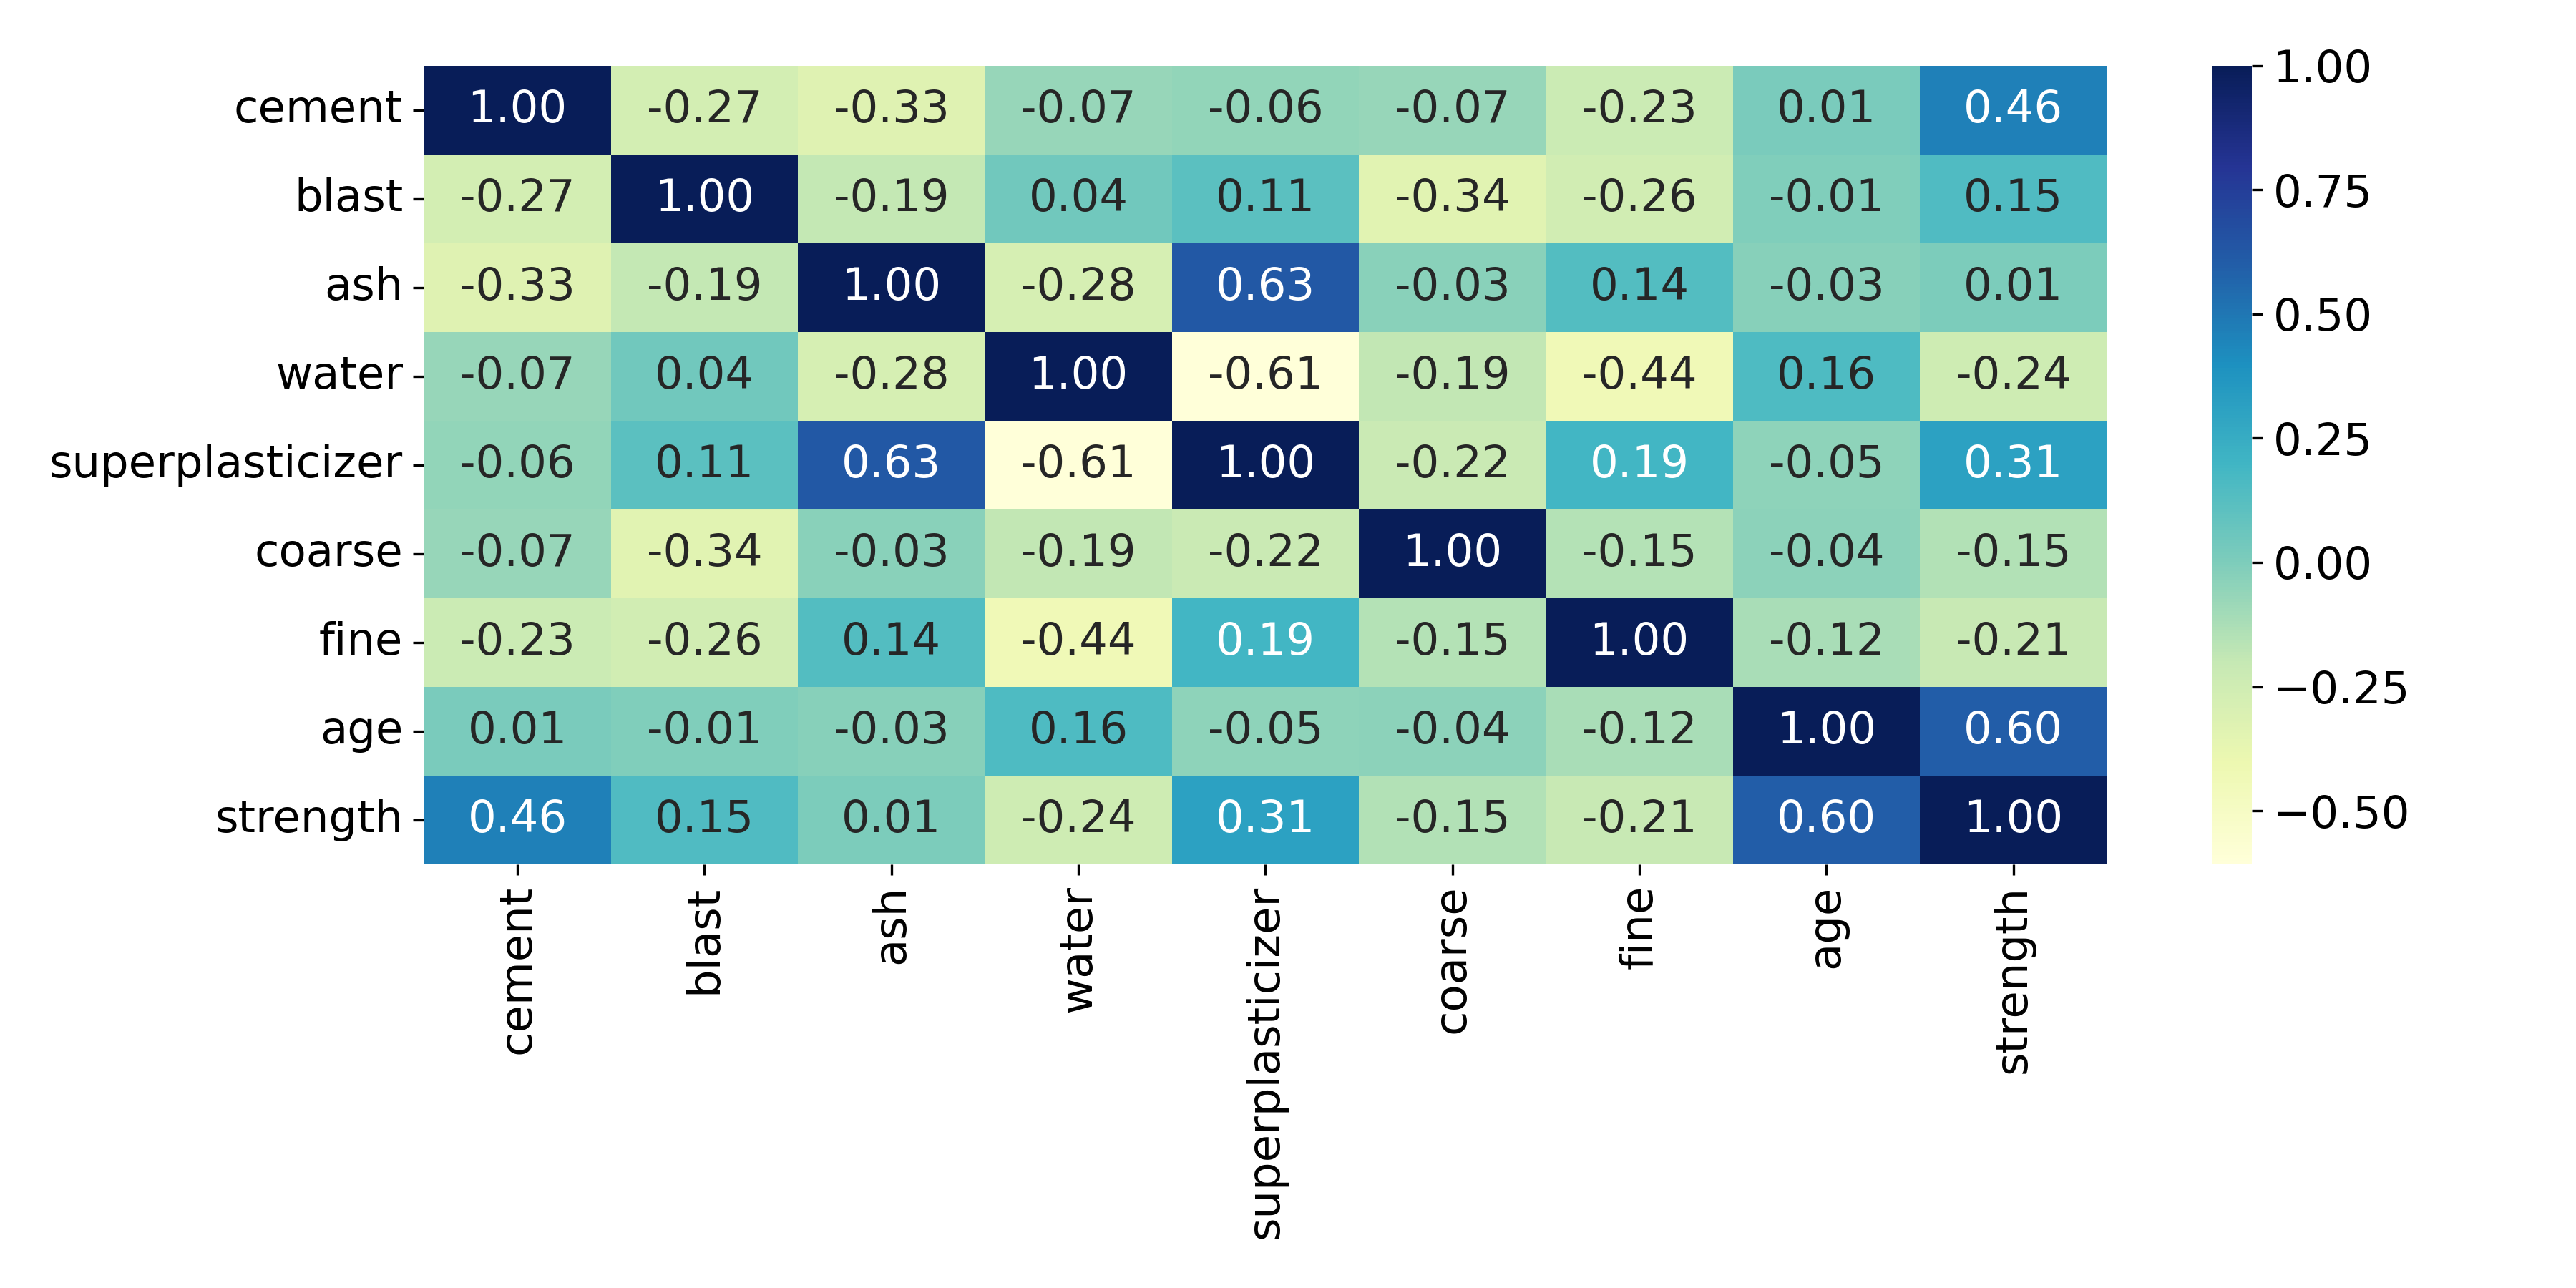
\includegraphics[width=1\textwidth]{../scripts/images/corr.png}
    Quelle: Eigene Darstellung, \ref{linreg}.
    \label{pic:corr}
\end{figure}

\section{Modellierung der linearen Regression}

TODO: Modell fitten

\begin{figure}[h]
    \caption{Residuenanalyse: Beziehung zwischen Vorhersagen und Abweichungen.}
    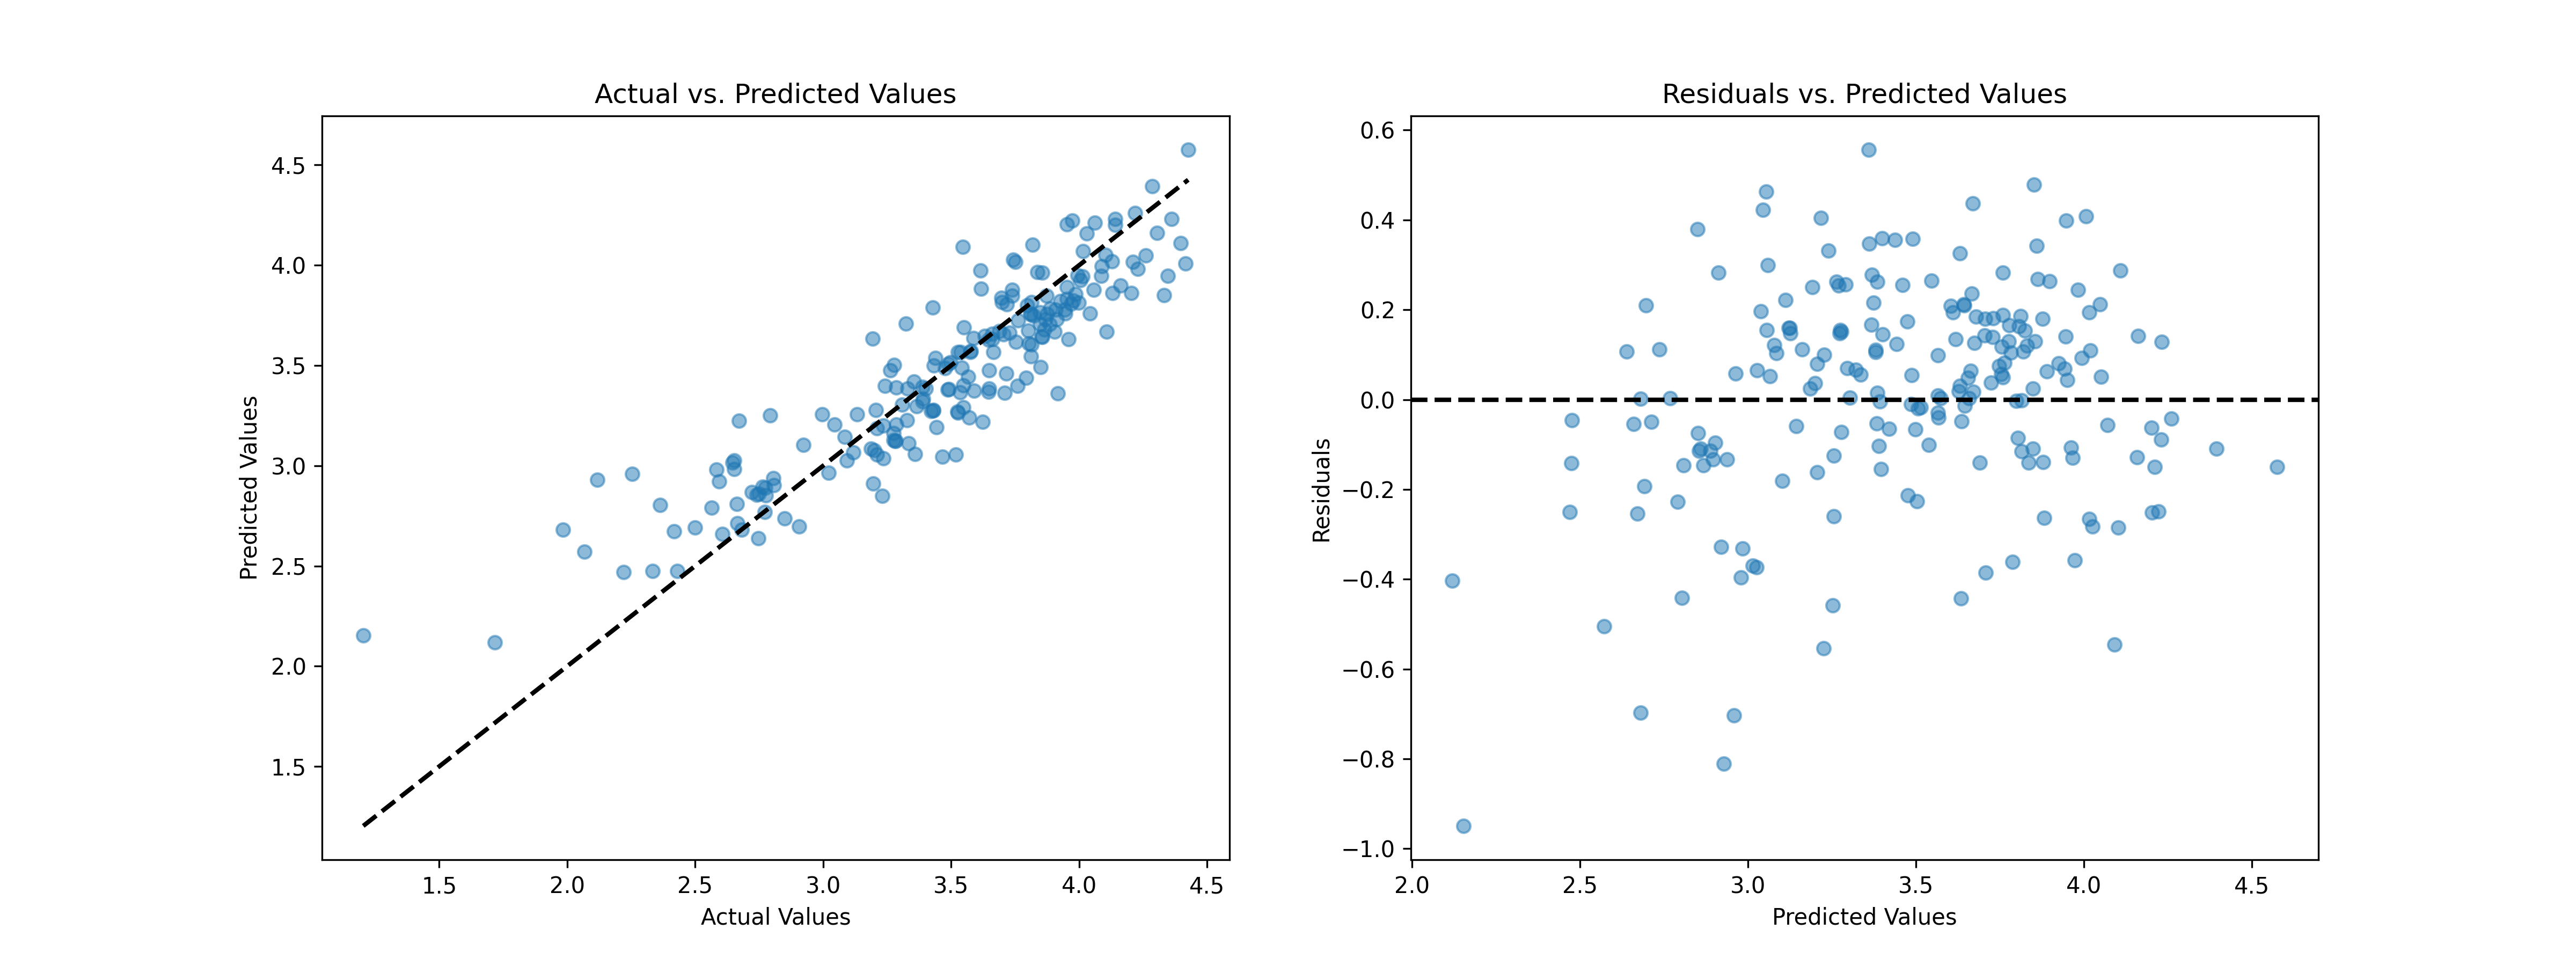
\includegraphics[width=1\textwidth]{../scripts/images/residuals.png}
    Quelle: Eigene Darstellung, \ref{linreg}.
    \label{pic:residuals}
\end{figure}